\name{glogsp}{draw a log spectrum graph}{plotting graphs}

\begin{synopsis}
\item[glogsp] [ --O $O$ ] [ --x $X$ ] [ --y $ymin \; ymax$ ] [ --ys $YS$ ] 
              [ --p $P$ ] [ --ln $LN$ ] 
\item[\ ~~~~~~~] [ --s $S$ ] [ --l $L$ ] [ --c $comment$ ] [ {\em infile} ]
\end{synopsis}

\begin{qsection}{DESCRIPTION}
This command reads input data from the starndard input in float format,
and plots its log spectrum.
This command can be used in connection with commands such as ``xgr''.
\par
Actually, it uses {\em fig} and {\em fdrw} commands through a
shell script.
\end{qsection}

\begin{options}
	\argm{O}{O}{origin of graph\\
		      \begin{minipage}{4.5cm}
		       \begin{tabular}{ccc}
			1 & ( 40,205) & [mm] \\
			2 & (125,205) & [mm] \\
			3 & ( 40,120) & [mm] \\
			4 & (125,120) & [mm] \\
			5 & ( 40, 35) & [mm] \\
			6 & (125, 35) & [mm]
		       \end{tabular}\\\hspace*{\fill}
		      \end{minipage}
		      \begin{minipage}{4.5cm}
		       \leavevmode
		       \includegraphics{fig/glogsp-on.eps}
		      \end{minipage}\\\hspace*{\fill}}{1}
	\argm{x}{X}{ $x$ scale��\\
		       \begin{tabular}{cl}
			1 & normalized frequency($0 \sim 0.5$) \\
			2 & normalized frequency($0 \sim \pi$) \\
			4 & frequency($0 \sim 4$kHz) \\
			5 & frequency($0 \sim 5$kHz) \\
			8 & frequency($0 \sim 8$kHz) \\
			10 & frequency($0 \sim 10$kHz) 
		       \end{tabular}\\\hspace*{\fill}}{1}
	\argm{y}{ymin \; ymax}{ $y$ scale[dB]}{0 100}
	\argm{ys}{YS}{ Y-axis scaling factor}{20}
	\argm{p}{P}{pen number($1 \sim 10$)}{1}
	\argm{ln}{LN}{kind of line style($0 \sim 5$) please refer to ``fig''
                      command section}{1}
	\argm{s}{S}{start frame number}{0}
	\argm{l}{L}{frame length}{256}
	\argm{c}{\rm comment}{coment for the graph}{N/A}
	\desc[1zh]{Usually, the options below do not need to be assigned.}
	\argm{W}{W}{width of the graph($\time 100$mm)}{0.6}
	\argm{H}{H}{height of the graph($\time 100$mm)}{0.6}
	\argm{v}{}{over write mode}{FALSE}
	\argm{o}{xo \; yo}{origin of the graph.
                      if -o option exists, -O is not effective}{40 205}
	\argm{g}{G}{type of frame of the graph($0 \sim 2$).
                    please refer to ``fig'' command section.}{2}
	\argm{f}{file}{additional data file for fig}{NULL}
	\argm{help}{}{print help in detail}{}
\end{options}

\begin{qsection}{EXAMPLE}
In the example below, speech data sampled at 10kHz is read
in short format from {\em data.s} file,
the magnitude of its log spectrum is evaluated and plotted on the screen:
\begin{quote}
 \verb!x2x +sf data.s | bcut -s 4000 -e 4255 | window -n 2| spec |\! \\
 \verb!glogsp -x 5 | xgr!
\end{quote}
\begin{center}
 \leavevmode
 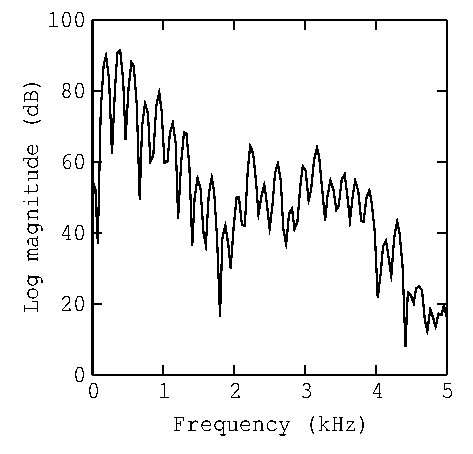
\includegraphics{fig/glogsp-sample.eps}
\end{center}
\end{qsection}

\begin{qsection}{SEE ALSO}
 fig, fdrw, xgr, psgr, grlogsp, gwave
\end{qsection}

